\begin{featurebox}
\caption{The Rules of Engagement for Order-Of-Magnitude Estimates}
This work relies heavily on so-called "back-of-the-envelope" estimates to
understand the growth-rate dependent abundances of molecular
complexes. This moniker arises from the limitation that any estimate should be
able to fit on the back of a postage envelope. Therefore, we must draw a set of
rules governing our precision and sources of key values.

\textbf{\itshape The rule of "one, few, and ten".} The philosophy behind
order-of-magnitude estimates is to provide a estimate of the appropriate scale,
not a prediction with infinite accuracy. As such, we define three different
scales of precision in making estimates. The scale of "one" is reserved for
values that range between 1 and 2. For example, If a particular process has been
experimentally measured to transport 1.87 protons for a process to occur, we approximate
this process to require 2 protons per event. The scale of "few" is reserved for
values ranging between 3 and 5. For example, we will often use Avogadro's number
to compute the number of molecules in a cell given a concentration and a volume.
Rather than using Avogadro's number as $6.02214 \times 10^{23}$, we will
approximate it as $5 \times 10^{23}$. Finally, the scale of "ten" is reserved
for values which we know within an order of magnitude. If a particular protein
complex is present at 883 copies per cell, we say that it is present in
approximately $10^3$ copies per cell. These different scales will be used
to arrive at simple estimates that report the expected scale of the
observed data. Therefore, the estimates  presented here should not be viewed as
hard-and-fast predictions of precise copy numbers, but as approximate lower (or upper)
bounds for the number of complexes that may be needed to satisfy some cellular requirement.

Furthermore, we use equality symbols ($=$) sparingly and frequently defer to
approximation ($\approx$) or scaling ($\sim$) symbols when reporting an
estimate. When $\approx$ is used, we are implicitly stating that
we are confident in this estimate within a factor of a few. When a scaling
symbol $\sim$ is used, we are stating that we are confident in our estimate to
within an order of magnitude.

\textbf{\itshape The BioNumbers Database as a source for values.} In making our
estimates, we often require approximate values for key cellular properties, such
as the elemental composition of the cell, the average dry mass, or approximate
rates of synthesis. We rely heavily on the BioNumbers Database \citep{milo2010}
as a repository for such information. Every value we draw from this database has
an associated BioNumbers ID number, abbreviated as BNID, and we provide this
reference in grey-boxes in each  figure.


\textbf{\itshape Uncertainty in the data sets and the accuracy of an estimate.}
The data sets presented in this work are the products of
careful experimentation with the aim to report, to the best of their ability,
the absolute copy numbers of proteins in the cell. These data, collected over
the span of a few years, come from different labs and use different internal
standards, controls, and even techniques (discussed further in Appendix \nameref{sec:SI_exp_summary}).
As a result, there is notable disagreement in the measured copy numbers for
some complexes across data sets. In assessing whether our estimates could explain the
observed scales and growth-rate dependencies, we also considered the degree of
variation between the different data sets. For example, say a particular
estimate undercuts the observed data by an order of magnitude. If all data sets
agree within a factor of a few of each other, we revisit our estimate and
consider what me may have missed. However, if the data sets themselves disagree
by an order of magnitude, we determine that our estimate is
appropriate given the variation in the data.
\label{box:estimate_rules}
\end{featurebox}


\section{Nutrient Transport}
We begin our series of estimates by considering the critical transport
processes diagrammed in \FIG{categories}(A). In order to build new cellular
mass, the molecular and elemental building blocks must be scavenged from the
environment in different forms. Carbon, for example, is acquired via the
transport of carbohydrates and sugar alcohols with some carbon sources
receiving preferential treatment in their consumption \citep{monod1947}.
Phosphorus, sulfur, and nitrogen, on the other hand, are harvested primarily
in the forms of inorganic salts, namely phosphate, sulfate, and ammonia
\citep{jun2018, assentoft2016, stasi2019, antonenko1997, rosenberg1977,
willsky1973}. All of these compounds have different permeabilities across the
cell membrane \citep{phillips2018} and most require some energetic investment
either via ATP hydrolysis or through the proton electrochemical gradient to
bring the material across the hydrophobic cell membrane.
% Given the diversity
% of biological transport mechanisms and the vast number of inputs needed to
% build a cell, we begin by considering transport of one of the most important
% cellular ingredients, carbon.

The elemental composition of \textit{E. coli} has received much quantitative
attention over the past half century \citep{neidhardt1991,
taymaz-nikerel2010, heldal1985, bauer1976}, providing us with a starting
point for estimating how many atoms of each element must be scavenged from
the environment. While there is some variability in the exact elemental
percentages (with different uncertainties), we can approximate the dry mass
of an \textit{E. coli} cell to be $\approx$ 45\% carbon (BioNumber ID:
100649, see \BOX{estimate_rules}), $\approx$ 15\% nitrogen (BNID: 106666),
$\approx$ 3\% phosphorus (BNID: 100653), and 1\% sulfur (BNID: 100655).
Here we use this stoichiometric breakdown to estimate the abundance and
growth rate dependence of a variety of transporters responsible for carbon
uptake, and provide more extensive investigation of the other critical elements --  phosphorus, sulfur,
and nitrogen -- in the Appendix \nameref{sec:SI_nutr_trans}.

 % and \FIGSUPP[carbon_tport]{phospho_sulfo}.


Using $\approx$ 0.3 pg as the typical \textit{E. coli} dry mass (BNID: 103904)
at a growth rate of $\approx$ 0.5 hr$^{-1}$, and nearly half of the dry mass
consisting of carbon, we estimate that $\sim 10^{10}$ carbon atoms must be
brought into the cell in order to double all of the carbon-containing molecules
(\FIG{carbon_tport}(A, top)). Typical laboratory growth conditions provide
carbon as a single class of sugar such as glucose, galactose, or xylose to name
a few. \textit{E. coli} has evolved myriad mechanisms by which these sugars can
be transported across the cell membrane. One such mechanism of transport is via
the PTS system which is a highly modular system capable of transporting a
diverse range of sugars \citep{escalante2012}. The glucose-specific component of
this system transports $\approx$ 200 glucose molecules per second per
transporter (BNID: 114686). Making the assumption that this is a typical sugar
transport rate, coupled with the need to transport $\sim 10^{10}$ carbon atoms,
we then expect on the order of 1000 transporters must be expressed in order to
bring in enough carbon atoms, diagrammed in the top panel of \FIG{carbon_tport}(A).
% This estimate, along with the observed average number of
% the PTS system carbohydrate transporters present in the proteomic data, is shown
% in \FIG{carbon_tport}(A).
While we estimate 1500 transporters are needed with a
5000 s division time, we can abstract this calculation to consider any
particular growth rate given knowledge of the cell density and volume as a
function of growth rate and direct the reader to the Appendix
\nameref{sec:SI_continuum_est} for more information. As revealed in
\FIG{carbon_tport}(A), experimental measurements exceed the estimate by several
fold, suggesting that transport of carbon into the cell is not rate limiting for
cell division. Abstracting this point estimate at 5000 s to a continuum of
growth rates (grey line in \FIG{carbon_tport}(A)) reveals an excess of
transporters even at faster growth rates. This constrasts with our observations
for uptake of phosphorus and sulfur, which align well with our expectations across
different growth conditions (\FIGSUPP[carbon_tport]{phospho_sulfo} and
discussed further in Appendix \nameref{sec:SI_nutr_trans})

\begin{figure}
    \begin{fullwidth}
    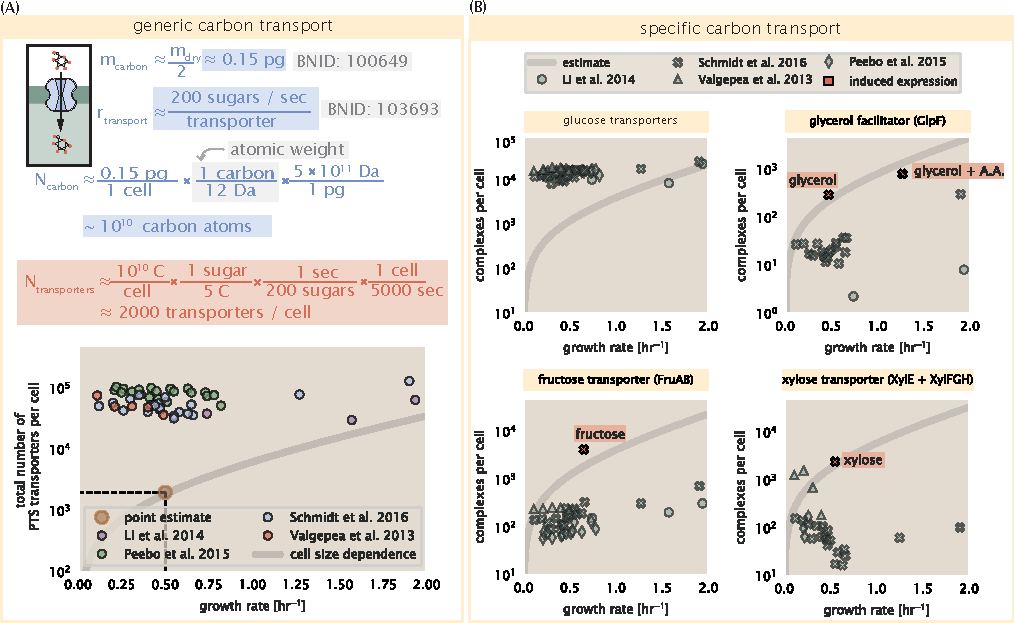
\includegraphics{main_figs/fig2_carbon_transport.pdf}
    \caption{\textbf{The abundance of carbon transport systems across growth
    rates.} (A) A simple estimate for the minimum number of generic carbohydrate
    transport systems (top) assumes $\sim 10^{10}$ C are needed to complete
    division, each transported sugar contains $\approx 5$ C, and each
    transporter conducts sugar molecules at a rate of $\approx 200$ per second.
    Bottom plot shows the estimated number of transporters needed at a growth
    rate of $\approx 0.5 $ per hr (light-brown point and dashed lines).  Colored
    points correspond to the mean number of complexes involved in carbohydrate import
    (complexes annotated with the Gene Ontology terms GO:0009401 and GO:0098704) for
    different growth conditions across different published datasets. (B) The
    abundance of various specific carbon transport systems plotted as a function
    of the population growth rate. The rates of substrate transport to compute
    the continuum growth rate estimate (grey line) were 200 glucose$\cdot$
    s$^{-1}$ (BNID: 103693),  2000 glycerol$\cdot$s$^{-1}$
    \citep{lu2003}, 200 fructose$\cdot$
    s$^{-1}$ (assumed to be similar to PtsI, BNID: 103693), and 50 xylose$\cdot$s$^{-1}$
    (assumed to be comparable to LacY, BNID:103159).
    Red points and highlighted text indicate conditions in
    which the
    only source of carbon in the growth medium induces expression of the
    transport system. Grey line in (A) and (B) represents the estimated number of transporters per cell at a continuum
    of growth rates.}\label{fig:carbon_tport}
    \figsupp[Estimates and observed abundances of phosphate and sulfate transporters.]{(A) Estimate for the
    number of PitA phosphate transport systems needed to maintain a 3\%
    phosphorus \textit{E. coli} dry mass. Points in plot correspond to
    the the total number of PitA transporters per cell. (B) Estimate of
    the number of CysUWA complexes necessary to maintain a 1\% sulfur
    \textit{E. coli} dry mass. Points in plot correspond to average
    number of CysUWA transporter complexes that can be formed given the
    transporter stoichiometry [CysA]$_2$[CysU][CysW][Sbp/CysP]. Grey line
    in (A) and (B) represents the estimated number of transporters per
    cell at a continuum of growth rates.}{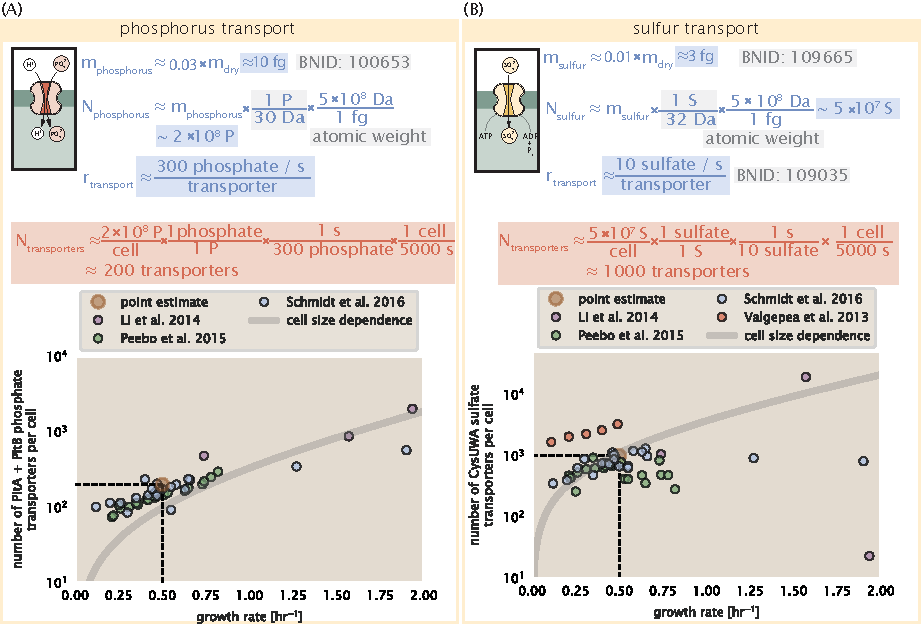
\includegraphics{main_figs/fig3_phospho_sulfo_transport.pdf}}\label{figsupp:phospho_sulfo}
    \end{fullwidth}
\end{figure}

The estimate presented in \FIG{carbon_tport}(A) neglects any specifics of the
regulation of the carbon transport system and the data shows how many
carbohydrate transporters are present on average. Using the diverse array of
growth conditions available in the data, we also explore how individual carbon
transport systems depend on specific carbon availability. In
\FIG{carbon_tport}(B), we show the total number of carbohydrate transporters
specific to different carbon sources. A striking observation, shown in the
top-left plot of \FIG{carbon_tport}(B), is the constancy in the expression of
the glucose-specific transport systems. Additionally, we note that the total
number of glucose-specific transporters is tightly distributed at $\approx 10^4$
per cell, the approximate number of transporters needed to sustain rapid growth
of several divisions per hour. This illustrates that \textit{E. coli} maintains
a substantial number of complexes present for transporting glucose regardless of
growth condition, which is known to be the preferential carbon source
\citep{monod1947, liu2005a, aidelberg2014}.

Many metabolic operons are regulated with dual-input logic gates that are only
expressed when glucose concentrations are low (mediated by cyclic-AMP receptor
protein CRP) and the concentration of other carbon sources are elevated
\citep{gama-castro2016, zhang2014a, gama-castro2016, belliveau2018, ireland2020}.
% A famed example of such dual-input
% regulatory logic is in the regulation of the \textit{lac} operon which is only
% activated in the absence of glucose and the presence of allolactose, an
% intermediate in lactose metabolism \citep{jacob1961}, though we now know of many
% other such examples \citep{ireland2020, gama-castro2016, belliveau2018}.
Several examples are shown in \FIG{carbon_tport}(B). Points colored in red
(labeled by red text-boxes) correspond to growth conditions in which the
specific carbon source (glycerol, xylose, or fructose) is present. The grey
lines in \FIG{carbon_tport}(B) show the estimated number of transporters needed
at each growth rate to satisfy the cellular carbon requirement, adjusted for the
specific carbon source. These plots show that, in the absence of the particular
carbon source, expression of the transporters is maintained on the order of
$\sim 10^2$ per cell.
% However, when the transport substrate is present,
% expression is induced and the transporters become highly-expressed.
The low but non-zero abundances may  reflect the specific regulatory logic
involved, requiring that cells are able to transport some minimal amount of an
alternative carbon source in order to induce expression of these alternative
carbon-source systems.

% Together, this generic estimation and the specific examples of induced
% expression suggest that transport of carbon across the cell membrane, while
% critical for growth, is not the rate-limiting step of cell division.
If acquisition of nutrients was the limiting process in cell division under
typical growth conditions, could expression simply be increased to accommodate
faster growth? A way to approach this question is to compute the amount of space
in the bacterial membrane that could be occupied by nutrient transporters.
Considering a rule-of-thumb for the surface area of \textit{E. coli} of about 5
\textmu m$^2$ (BNID: 101792), we expect an areal density for 1000 transporters
to be approximately 200 transporters/ \textmu m$^2$. For a typical transporter
occupying about 50 nm$^2$/dimer, this amounts to about only 1 percent of the
total inner membrane \citep{szenk2017}. In addition, bacterial cell membranes
typically have densities of 10$^5$ proteins/\textmu m$^2$ \citep{phillips2018},
implying that the cell could accommodate more transporters if any one was rate limiting.
 % of a variety of
% species if it were rate limiting. As we will see in the next section, however,
% occupancy of the membrane can impose other limits on the rate of energy
% production.
%
